\documentclass[a4paper,11pt]{report}
\usepackage[T1]{fontenc}
\usepackage[utf8]{inputenc}
\usepackage{lmodern}
\usepackage{graphicx}
\usepackage[german]{babel}

\title{Funktionsweise eines Raycasters mithilfe eines selber geschriebenen Beispiels erkl\"art}
\author{Andreas Gwilt}

\begin{document}

\maketitle
\tableofcontents

\begin{abstract}
This looks rather concrete to me. Actually, no it doesn't.
\end{abstract}

\section{Was ist ein Raycaster?}
% say roughly what it is, and what i'm trying to do
Raycasting ist ein ziemlich weiter begriff, der meistens für eine Rendermethode benutzt wird. Allgemein ist es eine Technik, um zu sehen, ob ein Strahl eine Fläche schneidet. Man ``wirft'' einen Strahl, und überprüft, ob er eine Ebene schneidet oder nicht. Diese ist dem Raytracing sehr ähnlich, aber ist viel limitierter und auch schneller.

\begin{figure}[htbp] 
        \centering
        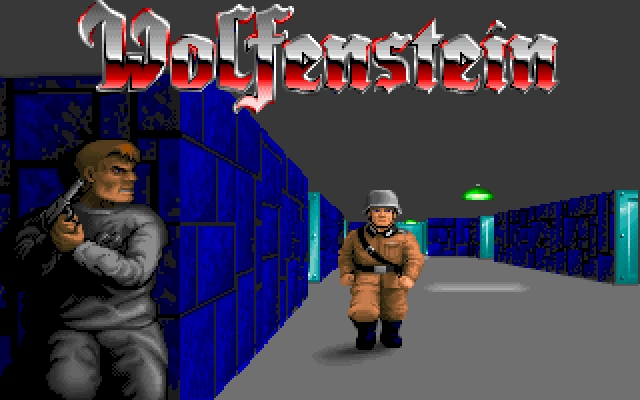
\includegraphics[width=4in]{wolfenstein-cover.jpg} 
        \caption{Wolfenstein 3D, ein Spiel, das einen Raycaster verwendete.}
\end{figure}

\subsection{Welche Probleme löst ein Raycaster?}
Raycasting ist eine Methode, um zu überprüfen, ob ein Strahl eine Fläche schneidet oder nicht. Die häufigste Anwendung dafür ist als einfaches Renderverfahren, um ein Spielfeld in pseudo-3D darzustellen. Es gibt aber auch mehrere andere Anwendungen, z.B. Kollisionserkennung oder um fest zu stellen, ob etwas sichtbar ist oder nicht. In meinem Beispiel nutze ich die Methode (in der \texttt{cast()} Funktion) hauptsächlich dazu, das Spielfeld darzustellen, aber auch als Kollisionserkennung für die \texttt{walk()} Funktion. Ich werde mich jedoch auf den Raycaster als Rendermethode konzentrieren. Raycasting wird auch meistens in Spielen benutzt, wo schnelles Rendern wichtig ist, da es als realistische Rendermethode nicht geeignet ist. \\
In den frühen 1990ern, als Raycasting beliebt wurde, hatte man noch ziemlich wenig Rechenleistung, wollte aber ``3D'' Spiele schreiben. Ein wirklich dreidimensionales Spiel-Engine (wie das 1996 erschienene Quake Engine) war noch nicht schnell genug, um in einem Spiel benutzt zu werden, also verwendete man Methoden wie Raycasting, um die Illusion von 3D herzustellen. Das vielleicht berühmteste Spiel, was Raycasting benutzte, war wahrscheinlich Wolfenstein 3D (Auch der erste beliebte Ego-Shooter). Wolfenstein 3D, auch Wolf3D genannt, hatte ein zweidimensionales Spielfeld, was in 3D dargestellt wurde. \\
Raycasting musste jedoch sehr viele Kompromisse eingehen, um so schnell zu sein. Das Spielfeld war ein zweidimensionales Array, also konnte es nur Rechte Winkel geben, und Decke und Boden mussten immer gleich hoch bleiben. Man erkennt an dem Screenshot von Wolf3D deutlich, dass das Spiel nicht wirklich dreidimensional ist. Auch sieht das Bild blockhaft aus, und die Beleuchtung ist nicht realistisch.

\subsection{Die Geschichte des Raycasters}
Raycasting wurde schon diskutiert, lang bevor PCs leistungsstark genug waren, um es wirklich in Spielen zu benutzen. Eine 1982 veröffentlichte Abhandlung von Scott Roth beschreibt Raycasting als Methode, dreidimensionale Körper zu rendern. \\
Einer der ersten Spiele, die das Prinzip implementierten, war \textit{Hovertank 3D}, was in April 1991 von id Software in einem Magazin veröffentlicht wurde. \textit{Hovertank 3D} war noch sehr primitiv und hatte noch keine Texturen auf den Wänden, noch dazu wurde es nicht zu einer großen Zielgruppe veröffentlicht, aber es war der Anfang einer neuen Genre von spielen. Im darauffolgenden November erschien \textit{Catacomb 3-D}, was Texturen hatte, und oft als der erste Ego-Shooter gesehen wird. \\
Zufrieden mit den zwei ``Prototypen'' entwickelten id Software ihr neues Spiel \textit{Wolfenstein 3D}, der die Technologie von \textit{Catacomb 3-D} übernahm. \textit{Wolfenstein 3D}, was 1992 von Apogee Software veröffentlicht wurde, war ein großer Erfolg und machte Ego-Shooter, und damit den Raycaster, bekannt. Danach schaffte id Software das revolutionäre Spiel \textit{DOOM}. \textit{DOOM} war ein noch viel größerer Erfolg, der einen sehr verbesserten Spiel-Engine hatte. Das neue Engine war jedoch nicht wirklich mehr ein echter Raycaster, sondern benutzte Binary Space Partitioning und andere fortgeschrittene Methoden.
\end{document}
